% $Header: /Users/joseph/Documents/LaTeX/beamer/solutions/generic-talks/generic-ornate-15min-45min.en.tex,v 90e850259b8b 2007/01/28 20:48:30 tantau $

\documentclass[xcolor=dvipsnames,notes]{beamer}

\mode<presentation>
{
  % \usetheme{Frankfurt}
  % or ...

  %\setbeamercovered{transparent}
  % or whatever (possibly just delete it)
}

\usepackage[english]{babel}
\usepackage[utf8]{inputenc}
\usepackage{times}
\usepackage[T1]{fontenc}
\usepackage{graphicx}
\usepackage{mathpartir}
%\usepackage[usenames,dvipsnames]{xcolor}

\beamertemplatenavigationsymbolsempty

\title[Formalizing \emph{TAPL} in Isabelle/HOL]
{Formalizing \emph{Types and Programming Languages} in Isabelle/HOL}
\author{Martin Desharnais}
\institute[ÉTS]{École de technologie supérieure}
\date{}

% If you have a file called "university-logo-filename.xxx", where xxx
% is a graphic format that can be processed by latex or pdflatex,
% resp., then you can add a logo as follows:

%\pgfdeclareimage[height=0.5cm]{university-logo}{logo-ETS}
%\logo{\pgfuseimage{university-logo}}



% Delete this, if you do not want the table of contents to pop up at
% the beginning of each subsection:
\AtBeginSection[]
{
  \begin{frame}<beamer>{Outline}
    \tableofcontents[currentsection,currentsubsection]
  \end{frame}
}


% If you wish to uncover everything in a step-wise fashion, uncomment
% the following command:

%\beamerdefaultoverlayspecification{<+->}


\begin{document}

\begin{frame}
  \titlepage
\end{frame}

\begin{frame}{Outline}
  \tableofcontents
  % You might wish to add the option [pausesections]
\end{frame}

\section{Motivations}

\begin{frame}{Why this book?}
  \begin{center}
    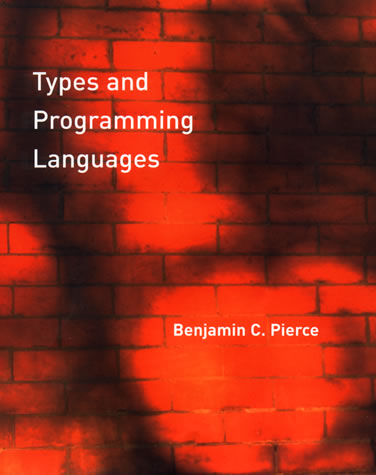
\includegraphics[scale=0.75]{TAPL.jpg}
  \end{center}
\end{frame}

\note[itemize]{
  \item Interested in programming languages and static verification
  \item \emph{TAPL} is onsidered as a reference on the subject
  \item \emph{TAPL} covers both $\lambda$-calculus and type systems
  \item \emph{TAPL} is very beginer friendly
  \item Asked my supervisor if he had it so I can borrow
  \item Was a good start to find a thesis subject
}

\begin{frame}{Why a formalization?}
  \begin{center}
    
\includegraphics[scale=0.2]{whiteboard_math.jpg} \\
    \vspace{20pt}
    Formalization = Definitions + Properties + Proofs \\
  \end{center}
\end{frame}

\note[itemize]{
  \item Validate pen \& paper proofs
  \item Clarifies corner cases
  \item Learning tool
}

\begin{frame}{Why in Isabelle/HOL?}
  \begin{center}
    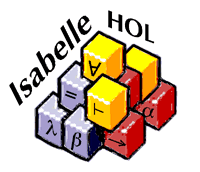
\includegraphics[scale=0.6]{isabelle_hol.png} \\
    \vspace{20pt}
    HOL = Functional Programming + Logic
  \end{center}
\end{frame}

\note[itemize]{
  \item Isabelle/HOL: interactive theorem prover based on HOL
  \item Isabelle/HOL: 2nd most used proof assistant (behind Coq)
  \item I contributed to the implementation in intership at TU München
  \item Local expertise available at the research chair
}

\section{Definition of the $\lambda$-Calculus}

\begin{frame}{What is the $\lambda$-calculus?}
  \begin{columns}[c]
    \column{0.4\textwidth}
      \begin{align*}
        t ::= & \\
          & x && \text{variable} \\
          & \lambda x. \; t && \text{abstraction} \\
          & t_1 \text{ } t_2 && \text{application}
      \end{align*}
    \column{0.6\textwidth}
      \begin{align*}
        & \lambda x. \; x \\
        & \lambda x. \lambda y. \; x \\
        & \lambda f. \lambda x. \; f \; x \; x \\
        & \lambda f. \lambda g. \lambda x. \; f \; (g \; x)
      \end{align*}
  \end{columns}
  \vspace{20pt}
  \begin{center}
    Variable names are irrelevent: \\
    $\lambda x. \; x \: = \: \lambda y. \; y$ \\
    \vspace{20pt}
    Function application: \\
    $(\lambda x. \; x \; x) \; y \: = \: y \; y$
  \end{center}
\end{frame}

\begin{frame}{Formalization of terms}
  \begin{center}
    \small
    \begin{align*}
      t ::= & \\
        & x && \text{variable} \\
        & \lambda x. \ t && \text{abstraction} \\
        & t_1 \text{ } t_2 && \text{application}
    \end{align*}\\
    \vspace{20pt}
    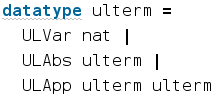
\includegraphics[scale=0.4]{term.png}
  \end{center}
\end{frame}

\begin{frame}{Formalization of single-step evaluation}
  \begin{center}
    \small
    \begin{displaymath}
      \inferrule {t_1 \implies t_1'}{t_1 \ t_2 \implies t_1' \ t_2}
    \end{displaymath}
    \begin{displaymath}
      \inferrule {t_2 \implies t_2'}{v_1 \ t_2 \implies v_1 \ t_2'}
    \end{displaymath}
    \begin{displaymath}
      \inferrule {}{(\lambda x. \ t_{12}) \ v_2 \implies [x \mapsto v_2] \ t_{12}}
    \end{displaymath}
    \vspace{20pt}
    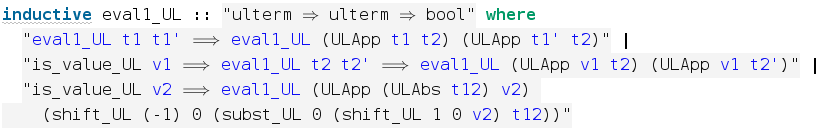
\includegraphics[scale=0.4]{eval1.png}
  \end{center}
\end{frame}

\begin{frame}{Formalization of multi-step evaluation}
  \begin{center}
    \small
    \begin{quotation}
      \noindent The \emph{multi-step evaluation} relation $\to^*$ is the reflexive, transitive closure
      of one-step evaluation. That is, it is the smallest relation such that (1) if t $t \to t'$ then
      $t \to^* t'$, (2) $t \to^* t$ for all $t$, and (3) if $t \to^* t'$ and $t' \to^* t''$, then
      $t \to^* t''$.
    \end{quotation}
    \vspace{20pt}
    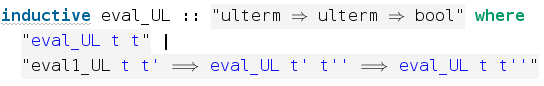
\includegraphics[scale=0.4]{eval.png}
  \end{center}
\end{frame}

\section{Augmenting $\lambda$-Calculus with a Type System}

\begin{frame}{What are type systems?}
  \begin{center}
    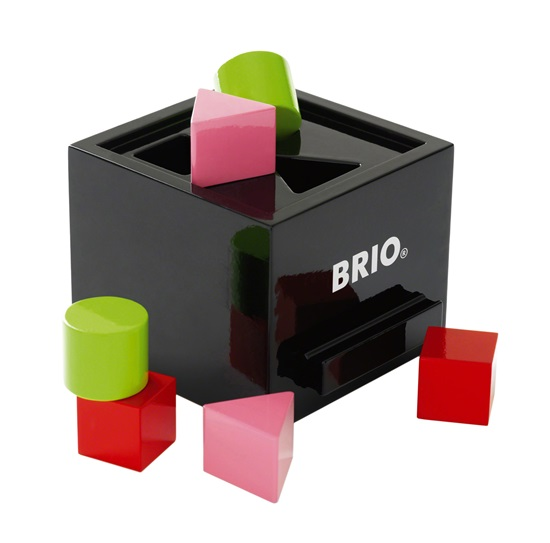
\includegraphics[scale=1]{shape_toy.jpg} \\
    Classification according to kind of values \\
    \bigskip
    \textcolor{OliveGreen}{Detection of errors \qquad Abstractions \qquad Maintenance} \\
    \textcolor{BrickRed}{Inflexible \qquad Restrictive}
  \end{center}
\end{frame}

\begin{frame}{Formalization of typing relation}
  \begin{center}
    \small
    \begin{displaymath}
      \inferrule {x : T \in \Gamma}{\Gamma \vdash x : T}
    \end{displaymath}
    \begin{displaymath}
      \inferrule {\Gamma, x : T_1 \vdash t_2 : T_2}
      {\Gamma \vdash \lambda x : T_1 . t_2 : T_1 \to T_2}
    \end{displaymath}
    \begin{displaymath}
      \inferrule {
        \Gamma \vdash t_1 : T_{11} \to T_{12} \\
        \Gamma \vdash t_2 : T_{11} \\
      }
      {\Gamma \vdash t_1 \ t_2 : T_{12}}
    \end{displaymath}
    \vspace{20pt}
    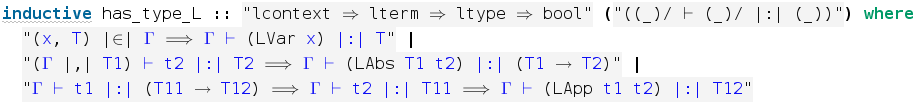
\includegraphics[scale=0.4]{has_type.png}
  \end{center}
\end{frame}

\section{Properties of the Typed $\lambda$-Calculus}

\begin{frame}{Type safety}
  \begin{center}
    
\includegraphics[scale=0.3]{hard_hat.png} \\
    \bigskip
    Safety = Progress + Preservation
  \end{center}
\end{frame}

\note[itemize]{
  \item Safety: A well-typed term always have a well-defined semantic.
    \begin{itemize}
      \item Semantic: values + evaluation relation
      \item C/C++ contains a lot of undefined behaviours
      \item e.g. accessing pass the end of an array
    \end{itemize}
  \item Progress: A well-typed term is not stuck (either it is a value or it can take a step
    according to the evaluation rules.
  \item Preservation: If a well-typed term takes a step of evaluation, then the resulting term is
    also well typed.
}

\begin{frame}{The progress theorem}
  \begin{center}
    \small
    \begin{quotation}
      \noindent Suppose $t$ is a closed, well-typed term (that is, $\vdash t : T$ for some
      $T$). Then either $t$ is a value or else there is some $t'$ with $t \to t'$.
    \end{quotation}
    \vspace{20pt}
    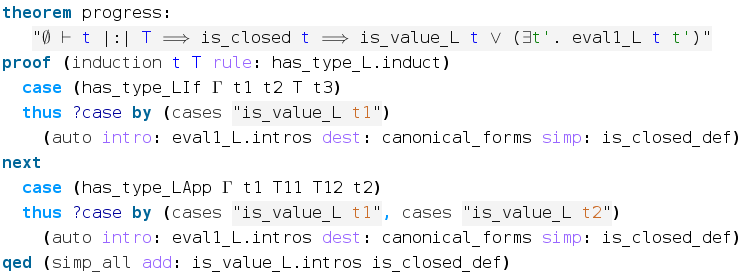
\includegraphics[scale=0.4]{progress.png}
  \end{center}
\end{frame}

\begin{frame}{Other theorems proved}
  \begin{itemize}
    \item Determinacy of evaluation
    \item Uniqueness of normal form
    \item (Non-)termination of evaluation
    \item Preservation of typing
    \item Erasability of types
    \item etc.
  \end{itemize}
\end{frame}

\section*{Summary}

\begin{frame}{What I learned}
  \begin{itemize}
    \item $\lambda$-calculus as core-calculus
    \item Type systems as security net
    \item Isabelle/HOL as developpement platform
    \item Formalization is as concrete as programming
    \item How my intership was relevent
  \end{itemize}
\end{frame}

\end{document}


